\documentclass{article}
\usepackage{tikz}
\usetikzlibrary{shapes.geometric, arrows, positioning, fit, backgrounds}

\begin{document}

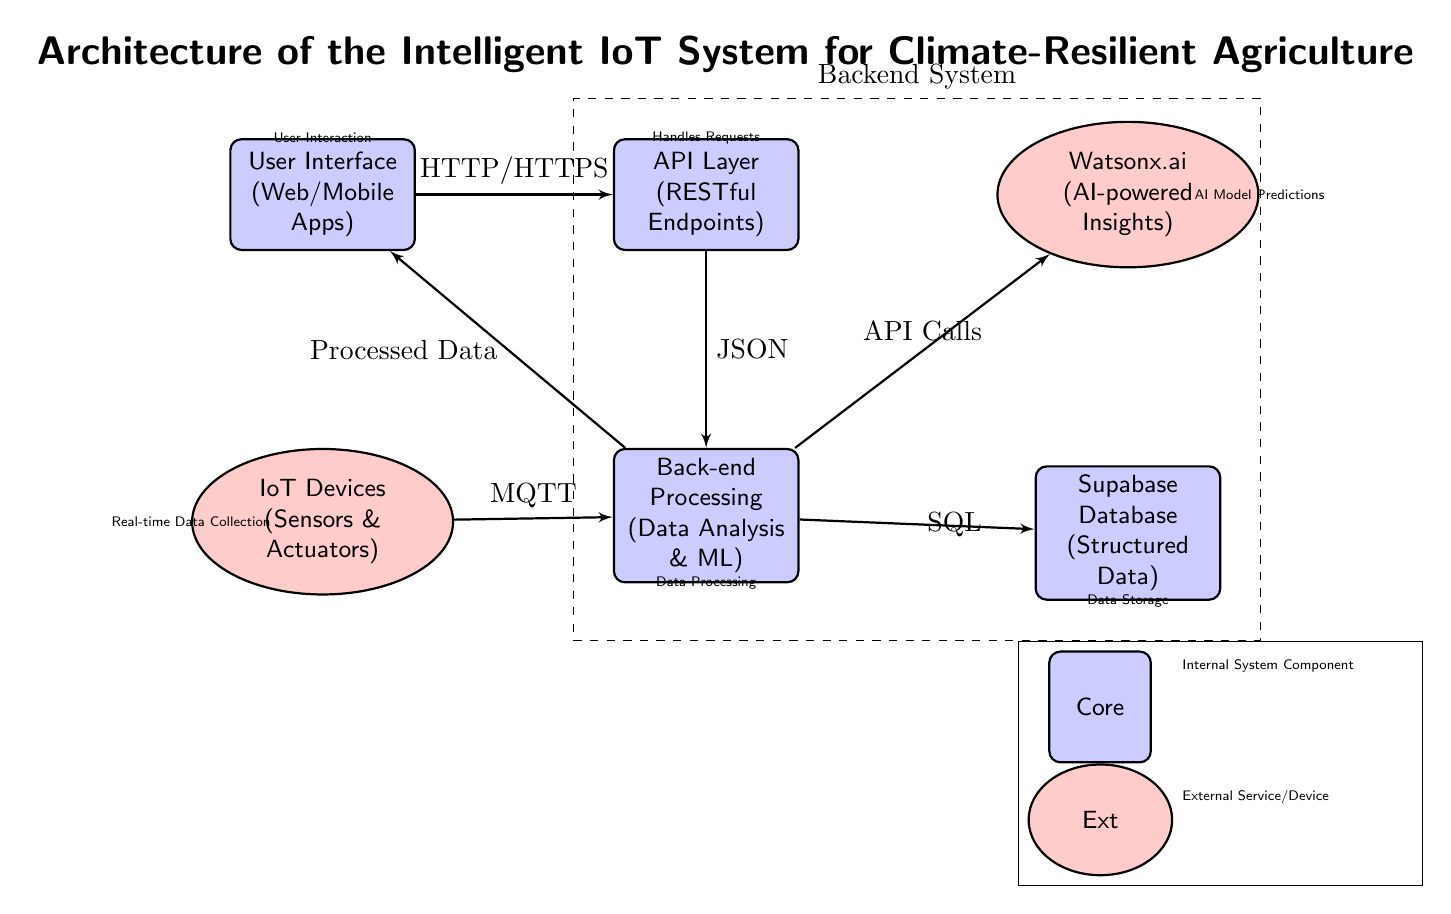
\begin{tikzpicture}[node distance=2.5cm, auto]

% Define improved styles
\tikzstyle{block} = [rectangle, draw=black, thick, fill=blue!20, 
    text width=6em, text centered, rounded corners, minimum height=4em, font=\small\sffamily]
\tikzstyle{cloud} = [ellipse, draw=black, thick, fill=red!20, 
    text width=6em, text centered, minimum height=4em, font=\small\sffamily]
\tikzstyle{line} = [draw, thick, -latex']
\tikzstyle{group} = [draw, dashed, inner sep=0.5cm]

% Place nodes
\node [block] (user) {User Interface \\ (Web/Mobile Apps)};
\node [block, right=of user] (api) {API Layer \\ (RESTful Endpoints)};
\node [block, below=of api] (backend) {Back-end Processing \\ (Data Analysis \& ML)};
\node [cloud, right=of api] (watsonx) {Watsonx.ai \\ (AI-powered Insights)};
\node [block, below=of watsonx] (database) {Supabase Database \\ (Structured Data)};
\node [cloud, below=of user] (iot) {IoT Devices \\ (Sensors \& Actuators)};

% Draw edges
\path [line] (user) -- node[midway, above] {HTTP/HTTPS} (api);
\path [line] (api) -- node[midway, right] {JSON} (backend);
\path [line] (backend) -- node[midway, above] {API Calls} (watsonx);
\path [line] (backend) -- node[midway, right] {SQL} (database);
\path [line] (iot) -- node[midway, above] {MQTT} (backend);
\path [line] (backend) -- node[midway, left] {Processed Data} (user);

% Add detailed labels
\node [text width=7em, text centered, font=\tiny\sffamily] at (user.north) {User Interaction};
\node [text width=7em, text centered, font=\tiny\sffamily] at (api.north) {Handles Requests};
\node [text width=7em, text centered, font=\tiny\sffamily] at (backend.south) {Data Processing};
\node [text width=7em, text centered, font=\tiny\sffamily] at (watsonx.east) {AI Model Predictions};
\node [text width=7em, text centered, font=\tiny\sffamily] at (database.south) {Data Storage};
\node [text width=7em, text centered, font=\tiny\sffamily] at (iot.west) {Real-time Data Collection};

% Group related components
\begin{pgfonlayer}{background}
    \node [group, fit=(api) (backend) (database), label=above:Backend System] {};
\end{pgfonlayer}

% Add title
\node [font=\Large\bfseries\sffamily] at (current bounding box.north) {Architecture of the Intelligent IoT System for Climate-Resilient Agriculture};

% Add legend
\matrix [draw, below left] at (current bounding box.south east) {
  \node [block, text width=3em] {Core}; & \node [text width=8em, align=left, font=\tiny\sffamily] {Internal System Component}; \\
  \node [cloud, text width=3em] {Ext}; & \node [text width=8em, align=left, font=\tiny\sffamily] {External Service/Device}; \\
};

\end{tikzpicture}

\end{document}
